\documentclass[calc1-main.tex]{subfiles}

\begin{document}
  \textbf{Problem:} Find a straight line $L$ that is tangent to a curve $C$ at a point $P$.

  \textsf{``For simplicity, restrict ourselves to curves which are graphs of functions.''}

  \textbf{How do we define the tangent line to a curve?}
  \begin{figure}[H]
    \centering
    \pgfplotsset{soldot/.style={color=blue,only marks,mark=*}}
\pgfplotsset{holdot/.style={color=blue,fill=white,only marks,mark=*}}

\begin{tikzpicture}
\begin{axis}[
ymin=-2.2,
ymax=.6,
xmin=.7,
xmax=3.4,
xtick = {2,3},
xticklabels = {$x_0$, $x_0+h$},
yticklabels = {,,},
axis lines = left
]
\addplot[domain=1:3.3,blue, very thick] {-(x-2)^2};
\draw[black, thick] (axis cs:1,0) -- (axis cs: 3,0);
\draw[black] (axis cs:1.5,.5) -- (axis cs: 3,-1);
\draw[black] (axis cs:1.5,0.4) -- (axis cs: 2.8,-0.64);
\draw[black] (axis cs:1.5,0.25) -- (axis cs: 2.5,-0.25);
% \draw[dotted] (axis cs:1,1) -- (axis cs:1,0);
\addplot[soldot] coordinates{(2,0)(2.5,-0.25)(2.8,-0.64)(3,-1)};
\node[above right] at (axis cs: 2,0) {$P$};
\node[right] at (axis cs: 3,-1) {$Q$};
\draw[dashed] (axis cs:2,0) -- (axis cs: 2,-3);
\draw[dashed] (axis cs:3,-1) -- (axis cs: 3,-3);
\end{axis}
\end{tikzpicture}

  \end{figure}

  The slope of the line PQ is
  \[
    \dfrac{f(x_0 + h) - f(x_0)}{h}.
  \]

  \begin{definition}
    Suppose $f$ is cts at $x=x_0$ and
    \[
      \lim_{h \to 0} \dfrac{f(x_0 + h) - f(x_0)}{h} = m
    \]
    If the limit exists, then the line with equation
    \[
      y = m(x - x_0) + f(x_0)
    \]
    is called \textbf{the tangent line} to the graph of $y=f(x)$ at $P = (x_0, f(x_0))$.
    If the limit does not exist and $m = \infty$ or $m = -\infty$ then the tangent line is the vertical line $x=x_0$.
    If the limit does not exist and is not $\pm \infty$ then there is no tangent line at $P$.
  \end{definition}

  \begin{example}
    Find an equation of the tangent line to the curve $y = x^2$ at $(1, 1)$.
  \end{example}
  \begin{solution}
    The slope is
    \[
      m = \lim_{h \to 0} \dfrac{f(1+h)-f(1)}{h} = 2.
    \]
    And an equation is $y=2(x-1)+1$.
  \end{solution}
  \begin{example}
    Find an equation of the tangent line to the curve $y = x^{1/3} = \sqrt[3]{x}$ at the origin.
  \end{example}
  \begin{solution}
    The slope of the tangent line is
    \[
      m = \lim_{h \to 0} \dfrac{h^{1/3}}{h} = \infty.
    \]
    So the tangent line is a vertical line $x=0$ (in other words the y-axis).
    \begin{figure}[H]
      \centering
      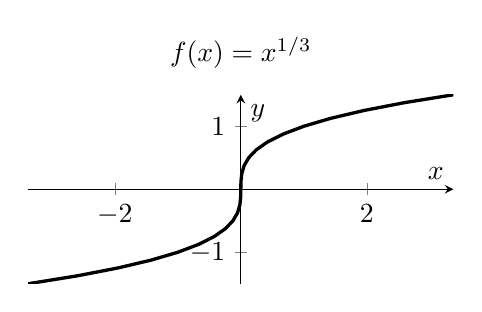
\begin{tikzpicture}
  \begin{axis}[
  axis lines=middle,
  x=8mm,
  y=8mm,
  title={$f(x)=x^{1/3}$},
  xlabel=$x$,
  ylabel=$y$]
  \addplot[domain=-1.5:1.5, very thick] ({x^3},{x});
\end{axis}
\end{tikzpicture}
    \end{figure}
  \end{solution}

\begin{remark}
  Tangent lines to curves such as circles and parabolas do not cross these curves, they just touch at a single point. However, for graphs of functions tangent lines may cross the curve such as above. In fact at inflection points (which we will define later) they always do! For example the tangent line to the graph of $f(x) = x^3$ at $x=0$ is the y-axis.
\end{remark}
  \begin{example}
    Does $f(x) = x^{2/3}$ have a tangent line at $(0, 0)$?
  \end{example}
  \begin{solution}
    The limit of the difference quotient is undefined at $0$since the right limit is $\infty$ while the left limit is $-\infty$. Hence the graph has no tangent line at $(0, 0)$.
    \begin{figure}[H]
      \centering
      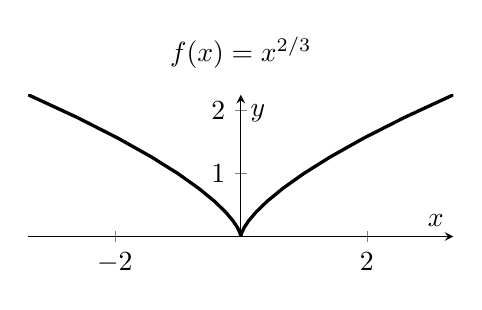
\begin{tikzpicture}
  \begin{axis}[
  axis lines=middle,
  x=8mm,
  y=8mm,
  title={$f(x)=x^{2/3}$},
  xlabel=$x$,
  ylabel=$y$]
  \addplot[domain=-1.5:1.5, very thick] ({x^3},{x^2});
\end{axis}
\end{tikzpicture}
    \end{figure}

    \textsf{``We say that this curve has a cusp at the origin. A cusp is an infinitely sharp point. If you were traveling along the curve, you would have to stop and turn 180$^{\circ}$ at the origin.''}
  \end{solution}

  \begin{example}
    Does $f(x) = \abs{x}$ have a tangent line at $(0, 0)$?
  \end{example}

  \begin{solution}
    The difference quotient is $\dfrac{\abs{h}}{h}$ which has right limit $1$ and left limit $-1$ at $h=0$.
    \begin{figure}[H]
      \centering
      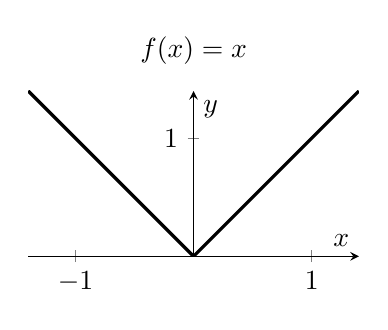
\begin{tikzpicture}
  \begin{axis}[
  axis lines=middle,
  xtick={-1,0,1},
  ytick={1},
  x=15mm,
  y=15mm,
  title={$f(x)=\abs{x}$},
  xlabel=$x$,
  ylabel=$y$]
  \addplot[domain=-1.4:0, very thick] {-x};
  \addplot[domain=0:1.4, very thick] {x};
\end{axis}
\end{tikzpicture}
    \end{figure}
  \end{solution}

\end{document}
